\begin{figure}[htbp]
	\centering
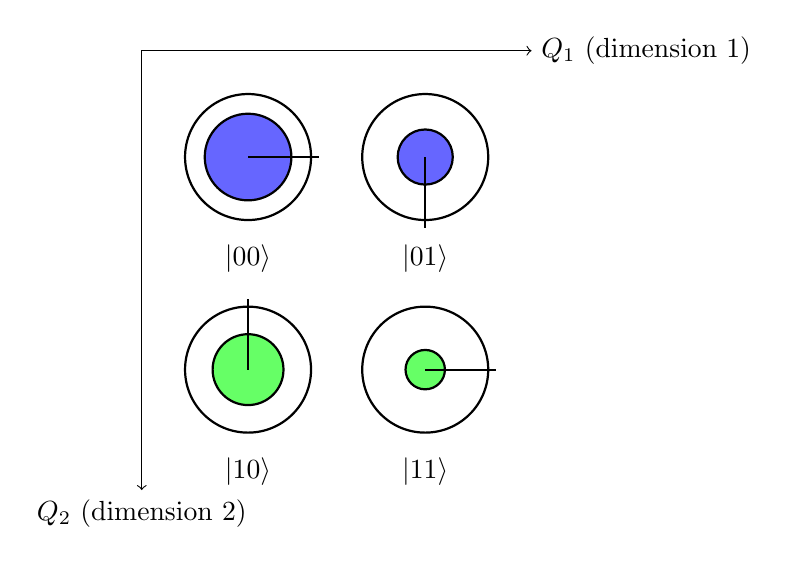
\begin{tikzpicture}[scale=0.9]
	\begin{scope}
		% 2x2 grid: top row |00>, |01>; bottom row |10>, |11>
		\foreach \x/\y/\label in {0/1.5/00, 2.5/1.5/01, 0/-1.5/10, 2.5/-1.5/11} {
			\node[draw, circle, minimum size=1.6cm, thick] at (\x,\y) {};
		}
		% Inner filled circles
		\foreach \x/\y/\fill/\r in {0/1.5/blue!60/1.1, 2.5/1.5/blue!60/0.7, 0/-1.5/green!60/0.9, 2.5/-1.5/green!60/0.5} {
			\node[draw, circle, fill=\fill, minimum size=\r cm, thick] at (\x,\y) {};
		}

		% phase line for each circle
		\draw[thick, black] (0,1.5) -- (1,1.5);    % 00
		\draw[thick, black] (2.5,1.5) -- (2.5,0.5); % 01
		\draw[thick, black] (0,-1.5) -- (0,-0.5);    % 10
		\draw[thick, black] (2.5,-1.5) -- (3.5,-1.5); % 11


		% Labels below each circle
		\node[below] at (0,1.5-1.1) {$|00\rangle$};
		\node[below] at (2.5,1.5-1.1) {$|01\rangle$};
		\node[below] at (0,-1.5-1.1) {$|10\rangle$};
		\node[below] at (2.5,-1.5-1.1) {$|11\rangle$};
	\end{scope}
	
	% Q1 axis (horizontal, left-right) on top of circles
	\draw[->] (-1.51,3.0) -- (4.0,3.0) node[right] {$Q_1$ (dimension 1)};
	% Q2 axis (vertical, top-to-bottom) left of circles
	\draw[->] (-1.5,3.0) -- (-1.5,-3.2) node[below] {$Q_2$ (dimension 2)};
	
	\end{tikzpicture}
	\caption{Two-qubit state in Dimensional Circular Notation. Circles are arranged in a $2 \times 2$ grid with explicit dimensional axes $Q_1$ and $Q_2$, corresponding to the two qubits. Two-qubit DCN: Circles arranged in 2D space with one dimension per qubit.}
	\label{fig:dcn-2qubit}
\end{figure}
